%!TEX root = ../thesis.tex

%%%%% Chapter: System Architecture %%%%%
\chapter{System Hyperparameters}

\ifpdf
    \graphicspath{{Chapter4/Figs/Raster/}{Chapter4/Figs/PDF/}{Chapter4/Figs/}}
\else
    \graphicspath{{Chapter4/Figs/Vector/}{Chapter4/Figs/}}
\fi


\section{Overview}


%%% Tesseract OCR %%%
\section{Tesseract OCR}

\subsection{Multi-scale Page Layout Analysis}

Recall that the Page Layout Analysis of the Tesseract OCR engine is able to identify distinct blocks (or bounding-boxes) of text by analysing the general layout of the input document. The Tesseract engine can provide different sets of bounding boxes at 5 scales: word, line, paragraph, block and page.

\Cref{fig:tess-pla-scales} shows the Tesseract output bounding-boxes at 4 different scales, excluding the `page' scale since the output of the `page' scale just contains one bounding-box which is the image boundary.

\begin{figure}[!htb]
  \centering
  \begin{subfigure}{.45\textwidth}
    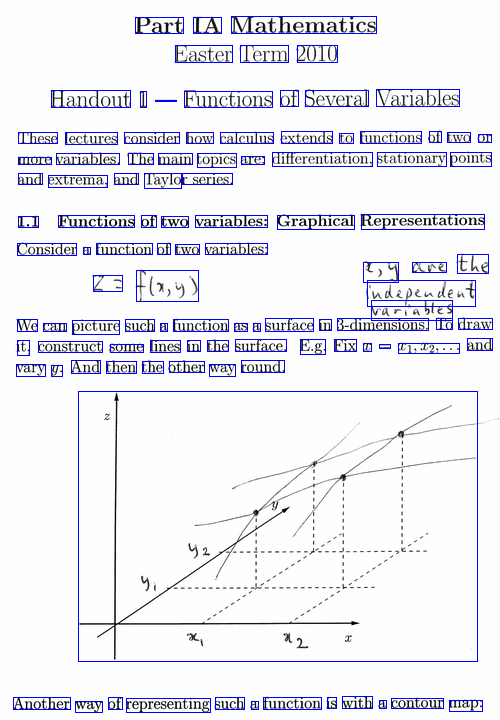
\includegraphics[width=\textwidth]{pla-word.png}
    \caption{Word scale}
  \end{subfigure}%
  \qquad
  \begin{subfigure}{.45\textwidth}
    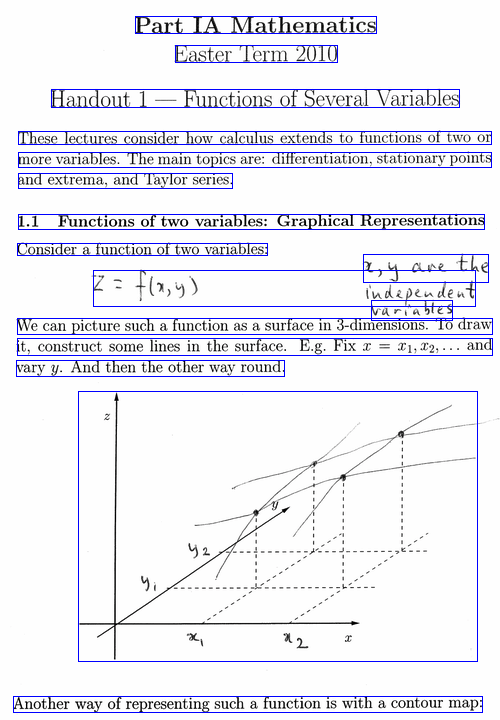
\includegraphics[width=\textwidth]{pla-line.png}
    \caption{Line scale}
  \end{subfigure}
  \vskip\baselineskip
  \begin{subfigure}{.45\textwidth}
    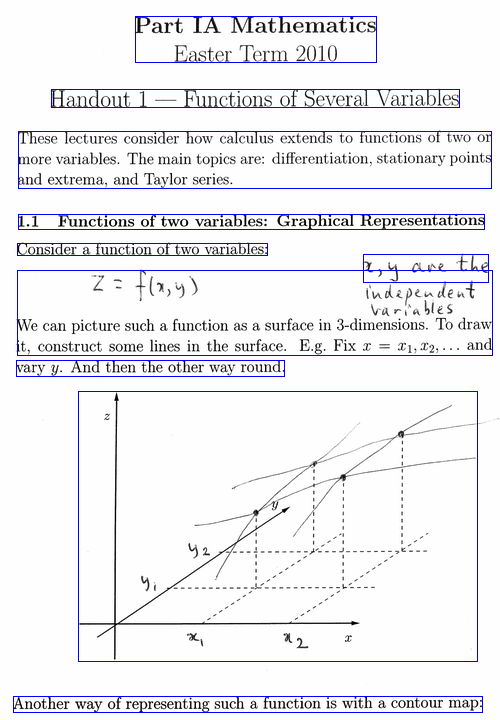
\includegraphics[width=\textwidth]{pla-par.png}
    \caption{Paragraph scale}
  \end{subfigure}%
  \qquad
  \begin{subfigure}{.45\textwidth}
    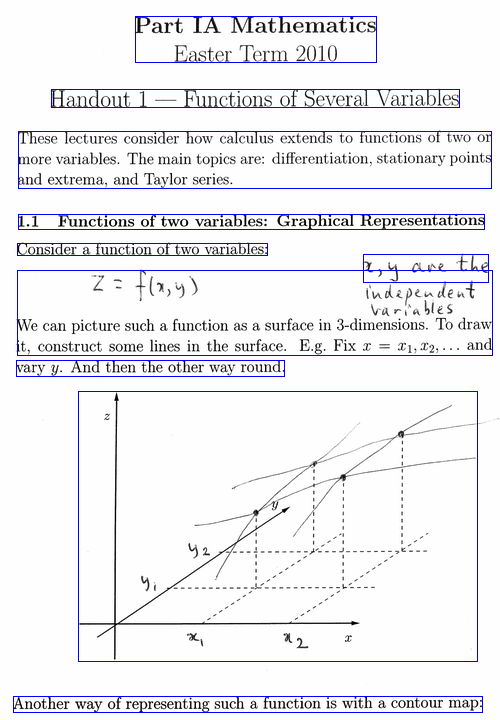
\includegraphics[width=\textwidth]{pla-block.png}
    \caption{Block scale}
  \end{subfigure}
  \caption{Different scales of Tesseract PLA}
  \label{fig:tess-pla-scales}
\end{figure}

In the actual system implementation, the user would be able to choose 4 different scales: word, line, paragraph and page. The `block' scale is removed from the implementation since in practice the difference between the `block' scale and the `paragraph' scale is negligible (which can be seen from \Cref{fig:tess-pla-scales}), and we keep the `paragraph' scale since the name `paragraph' is less ambiguous than `block'. 

We also keep the `page' scale in the system implementation for evaluation purposes described in later chapters, though this scale is not actually useful in practical use. The choice of PLA scale is considered to be one of the system hyperparameters.

\subsection{Model Switching}

Tesseract provides a large number of different models to support text recognition of different human languages. The default model is for recognising English text, which is named as \texttt{eng} in the Tesseract specification. 

Tesseract allows us to fine-tune existing models to produce improved models, or retrain from scratch to make completely new models. In this project, we have fine-tuned the default English model using additional handwritten data, and have included the fine-tuned model in the system implementation. The training of Tesseract OCR is further discussed in later chapters. 

Tesseract also allows us to specify what model to use before running the OCR engine. Using different models will eventually generate different recognition results. Therefore, the choice of the working Tesseract model is also one of the system hyperparameters.


\section{\texttt{diff}-based Alignment Algorithm}

\subsection{Problem Formulation}

Let $X$ = $X_1^n$ = ($X_1$,$X_2$,\ldots,$X_n$) and $Y$ = $Y_1^n$ = ($Y_1$,$Y_2$,\ldots,$Y_m$) be two sequences of symbols where $X_i \in A$ and $Y_j \in B$ for all $i$ and $j$. The sets $A$ and $B$ are also called \textit{alphabets}. Let $\phi$ be the `null symbol' which satisfies $\phi \notin A$ and $\phi \notin B$. Let $A^*$ = $A\cup\{\phi\}$ and $B^*$ = $B\cup\{\phi\}$.

Let $Z$ = $Z_1^p$ = ($Z_1$,$Z_2$,\ldots,$Z_p$), where $Z_i$ = $(S_i, T_i)$. Denote $S$ = $S_1^p$ = ($S_1$,$S_2$,\ldots,$S_p$) and $T$ = $T_1^p$ = ($T_1$,$T_2$,\ldots,$T_p$). We say $Z$ is an \textit{alignment} of sequences $X$ and $Y$ if:
\begin{enumerate}
  \item $Z_i \in A^* \times B^*$ and $Z_i \neq (\phi,\phi)$ for all $i$
  \item $X$ can be made equal to $S$ by inserting 0 or more null symbols $\phi$
  \item $Y$ can be made equal to $T$ by inserting 0 or more null symbols $\phi$
\end{enumerate}

Now define the Joint Weight Function, $\mathcal{F}(\cdot,\cdot)$: $A^* \times B^* \to \mathbb{R}$. The \textit{optimal alignment} $Z_{opt}$ is the alignment that maximise the sum of the joint weights, $\mathcal{W}$:
\begin{equation}
  Z_{opt} \,=\, \argmax_{Z} \mathcal{W}(Z) \,=\, \argmax_{Z} \sum_{i=1}^{p} \mathcal{F}(S_i,T_i)
\end{equation}
where $p$ denotes the length of $Z$ and may vary when $Z$ changes.

\subsection{Example: DNA Sequences}

In bioinformatics we often need to align different DNA sequences. To illustrate the above formulation, we use two example DNA sequences $X$ = \texttt{GCATGCT} and $Y$ = \texttt{GATTACA} with alphabets $A$ = $B$ = \{\texttt{A}, \texttt{T}, \texttt{G}, \texttt{C}\}. An example alignment could be:
\begin{center}
  \texttt{GCATG-CT}\\
  \texttt{G-ATTACA}
\end{center}
we can use $Z$ = (
  (\texttt{G},\texttt{G}),
  (\texttt{C},$\phi$),
  (\texttt{A},\texttt{A}),
  (\texttt{T},\texttt{T}),
  (\texttt{G},\texttt{T}),
  ($\phi$,\texttt{A}),
  (\texttt{C},\texttt{C}),
  (\texttt{T},\texttt{A})
) to express this alignment using the above formulation.

Usually when comparing two sequences, we care about the total weight (or score) of converting the first sequence to the second sequence by three basic operations: \textit{insertion}, \textit{deletion} and \textit{substitution}. These could be actually reflected in the Joint Weight Function $\mathcal{F}$:
\[
  \begin{cases}
    \mathcal{F}(\phi,y) & \text{\quad insert } y \text{ into } X \\
    \mathcal{F}(x,\phi) & \text{\quad delete } x \text{ from } X \\
    \mathcal{F}(x,y) & \text{\quad substitute } x \text{ with } y
  \end{cases}
\]
In the alignment of DNA sequences, it's common to assign positive scores for matches and negative scores for mismatches. If we define $\mathcal{F}(x,y)$ to be +1 if $x$ = $y$ and -1 otherwise, the total weight (or score) $\mathcal{W}$ can be calculated as:
\[ \mathcal{W}(Z) = 1 - 1 + 1 + 1 - 1 - 1 + 1 - 1 = 0 \]

\subsection{Alignment in the System}

In our system, we are working on 

\section{The Baseline System}



\nomenclature[z-JWF]{JWF}{Joint Weight Function}